% Options for packages loaded elsewhere
\PassOptionsToPackage{unicode}{hyperref}
\PassOptionsToPackage{hyphens}{url}
%
\documentclass[10pt]{report}
\usepackage{amsmath,amssymb}
\usepackage{lmodern}
\usepackage{iftex}
\usepackage[margin=0.8in]{geometry}
\usepackage{times}
\linespread{1.5}
\usepackage{titlesec}
\usepackage{xcolor}
\titleformat{\chapter}{\bfseries\centering\Huge\color{blue}\titlerule[2pt]}{\thechapter.}{10pt}{\huge}[\color{blue}{\titlerule[2pt]}]
\titlespacing{\chapter}{0pt}{0pt}{20pt}

\titleformat{\section}{\bfseries\large}{\thesection.}{0.5em}{}
\titlespacing{\section}{0pt}{0pt}{20pt}
\ifPDFTeX
  \usepackage[T1]{fontenc}
  \usepackage[utf8]{inputenc}
  \usepackage{textcomp} % provide euro and other symbols
\else % if luatex or xetex
  \usepackage{unicode-math}
  \defaultfontfeatures{Scale=MatchLowercase}
  \defaultfontfeatures[\rmfamily]{Ligatures=TeX,Scale=1}
\fi
% Use upquote if available, for straight quotes in verbatim environments
\IfFileExists{upquote.sty}{\usepackage{upquote}}{}
\IfFileExists{microtype.sty}{% use microtype if available
  \usepackage[]{microtype}
  \UseMicrotypeSet[protrusion]{basicmath} % disable protrusion for tt fonts
}{}
\makeatletter
\@ifundefined{KOMAClassName}{% if non-KOMA class
  \IfFileExists{parskip.sty}{%
    \usepackage{parskip}
  }{% else
    \setlength{\parindent}{0pt}
    \setlength{\parskip}{6pt plus 2pt minus 1pt}}
}{% if KOMA class
  \KOMAoptions{parskip=half}}
\makeatother
\usepackage{xcolor}
\usepackage[margin=1in]{geometry}
\usepackage{color}
\usepackage{fancyvrb}
\newcommand{\VerbBar}{|}
\newcommand{\VERB}{\Verb[commandchars=\\\{\}]}
\DefineVerbatimEnvironment{Highlighting}{Verbatim}{commandchars=\\\{\}}
% Add ',fontsize=\small' for more characters per line
\usepackage{framed}
\definecolor{shadecolor}{RGB}{248,248,248}
\newenvironment{Shaded}{\begin{snugshade}}{\end{snugshade}}
\newcommand{\AlertTok}[1]{\textcolor[rgb]{0.94,0.16,0.16}{#1}}
\newcommand{\AnnotationTok}[1]{\textcolor[rgb]{0.56,0.35,0.01}{\textbf{\textit{#1}}}}
\newcommand{\AttributeTok}[1]{\textcolor[rgb]{0.77,0.63,0.00}{#1}}
\newcommand{\BaseNTok}[1]{\textcolor[rgb]{0.00,0.00,0.81}{#1}}
\newcommand{\BuiltInTok}[1]{#1}
\newcommand{\CharTok}[1]{\textcolor[rgb]{0.31,0.60,0.02}{#1}}
\newcommand{\CommentTok}[1]{\textcolor[rgb]{0.56,0.35,0.01}{\textit{#1}}}
\newcommand{\CommentVarTok}[1]{\textcolor[rgb]{0.56,0.35,0.01}{\textbf{\textit{#1}}}}
\newcommand{\ConstantTok}[1]{\textcolor[rgb]{0.00,0.00,0.00}{#1}}
\newcommand{\ControlFlowTok}[1]{\textcolor[rgb]{0.13,0.29,0.53}{\textbf{#1}}}
\newcommand{\DataTypeTok}[1]{\textcolor[rgb]{0.13,0.29,0.53}{#1}}
\newcommand{\DecValTok}[1]{\textcolor[rgb]{0.00,0.00,0.81}{#1}}
\newcommand{\DocumentationTok}[1]{\textcolor[rgb]{0.56,0.35,0.01}{\textbf{\textit{#1}}}}
\newcommand{\ErrorTok}[1]{\textcolor[rgb]{0.64,0.00,0.00}{\textbf{#1}}}
\newcommand{\ExtensionTok}[1]{#1}
\newcommand{\FloatTok}[1]{\textcolor[rgb]{0.00,0.00,0.81}{#1}}
\newcommand{\FunctionTok}[1]{\textcolor[rgb]{0.00,0.00,0.00}{#1}}
\newcommand{\ImportTok}[1]{#1}
\newcommand{\InformationTok}[1]{\textcolor[rgb]{0.56,0.35,0.01}{\textbf{\textit{#1}}}}
\newcommand{\KeywordTok}[1]{\textcolor[rgb]{0.13,0.29,0.53}{\textbf{#1}}}
\newcommand{\NormalTok}[1]{#1}
\newcommand{\OperatorTok}[1]{\textcolor[rgb]{0.81,0.36,0.00}{\textbf{#1}}}
\newcommand{\OtherTok}[1]{\textcolor[rgb]{0.56,0.35,0.01}{#1}}
\newcommand{\PreprocessorTok}[1]{\textcolor[rgb]{0.56,0.35,0.01}{\textit{#1}}}
\newcommand{\RegionMarkerTok}[1]{#1}
\newcommand{\SpecialCharTok}[1]{\textcolor[rgb]{0.00,0.00,0.00}{#1}}
\newcommand{\SpecialStringTok}[1]{\textcolor[rgb]{0.31,0.60,0.02}{#1}}
\newcommand{\StringTok}[1]{\textcolor[rgb]{0.31,0.60,0.02}{#1}}
\newcommand{\VariableTok}[1]{\textcolor[rgb]{0.00,0.00,0.00}{#1}}
\newcommand{\VerbatimStringTok}[1]{\textcolor[rgb]{0.31,0.60,0.02}{#1}}
\newcommand{\WarningTok}[1]{\textcolor[rgb]{0.56,0.35,0.01}{\textbf{\textit{#1}}}}
\usepackage{graphicx}
\makeatletter
\def\maxwidth{\ifdim\Gin@nat@width>\linewidth\linewidth\else\Gin@nat@width\fi}
\def\maxheight{\ifdim\Gin@nat@height>\textheight\textheight\else\Gin@nat@height\fi}
\makeatother
% Scale images if necessary, so that they will not overflow the page
% margins by default, and it is still possible to overwrite the defaults
% using explicit options in \includegraphics[width, height, ...]{}
\setkeys{Gin}{width=\maxwidth,height=\maxheight,keepaspectratio}
% Set default figure placement to htbp
\makeatletter
\def\fps@figure{htbp}
\makeatother
\setlength{\emergencystretch}{3em} % prevent overfull lines
\providecommand{\tightlist}{%
  \setlength{\itemsep}{0pt}\setlength{\parskip}{0pt}}
\setcounter{secnumdepth}{-\maxdimen} % remove section numbering
\ifLuaTeX
  \usepackage{selnolig}  % disable illegal ligatures
\fi
\IfFileExists{bookmark.sty}{\usepackage{bookmark}}{\usepackage{hyperref}}
\IfFileExists{xurl.sty}{\usepackage{xurl}}{} % add URL line breaks if available
\urlstyle{same} % disable monospaced font for URLs
\hypersetup{
  pdftitle={Galamsey},
  pdfauthor={Boniface Kalong},
  hidelinks,
  pdfcreator={LaTeX via pandoc}}

\title{Galamsey}
\author{Boniface Kalong}
\date{7/2/2022}

\begin{document}
\maketitle

\begin{Shaded}
\begin{Highlighting}[]
\CommentTok{\#if(!require("pacman"))\{install.packages("pacman")\}}
\NormalTok{pacman}\SpecialCharTok{::}\FunctionTok{p\_load}\NormalTok{(}\AttributeTok{char =} \FunctionTok{c}\NormalTok{(}\StringTok{\textquotesingle{}rgee\textquotesingle{}}\NormalTok{,}\StringTok{\textquotesingle{}reticulate\textquotesingle{}}\NormalTok{,}\StringTok{\textquotesingle{}raster\textquotesingle{}}\NormalTok{,}\StringTok{\textquotesingle{}tidyverse\textquotesingle{}}\NormalTok{,}
                        \StringTok{\textquotesingle{}dplyr\textquotesingle{}}\NormalTok{,}\StringTok{\textquotesingle{}sf\textquotesingle{}}\NormalTok{,}\StringTok{\textquotesingle{}mapview\textquotesingle{}}\NormalTok{,}\StringTok{\textquotesingle{}mapeddit\textquotesingle{}}\NormalTok{,}\StringTok{\textquotesingle{}caret\textquotesingle{}}\NormalTok{,}\StringTok{\textquotesingle{}forcats\textquotesingle{}}\NormalTok{,}\StringTok{\textquotesingle{}reticulate\textquotesingle{}}\NormalTok{,}
                        \StringTok{\textquotesingle{}rgee\textquotesingle{}}\NormalTok{, }\StringTok{\textquotesingle{}remotes\textquotesingle{}}\NormalTok{, }\StringTok{\textquotesingle{}magrittr\textquotesingle{}}\NormalTok{, }\StringTok{\textquotesingle{}tigris\textquotesingle{}}\NormalTok{, }\StringTok{\textquotesingle{}tibble\textquotesingle{}}\NormalTok{, }\StringTok{\textquotesingle{}stars\textquotesingle{}}\NormalTok{, }\StringTok{\textquotesingle{}stars\textquotesingle{}}\NormalTok{,}
                        \StringTok{\textquotesingle{}st\textquotesingle{}}\NormalTok{, }\StringTok{\textquotesingle{}lubridate\textquotesingle{}}\NormalTok{, }\StringTok{\textquotesingle{}imputeTS\textquotesingle{}}\NormalTok{, }\StringTok{\textquotesingle{}leaflet\textquotesingle{}}\NormalTok{, }\StringTok{\textquotesingle{}classInt\textquotesingle{}}\NormalTok{, }\StringTok{\textquotesingle{}RColorBrewer\textquotesingle{}}\NormalTok{,}
                        \StringTok{\textquotesingle{}ggplot2\textquotesingle{}}\NormalTok{, }\StringTok{\textquotesingle{}googledrive\textquotesingle{}}\NormalTok{, }\StringTok{\textquotesingle{}geojsonio\textquotesingle{}}\NormalTok{, }\StringTok{\textquotesingle{}ggpubr\textquotesingle{}}\NormalTok{,}\StringTok{\textquotesingle{}cartogram\textquotesingle{}}\NormalTok{), }
               \AttributeTok{install =}\NormalTok{ F, }\AttributeTok{update =}\NormalTok{ F, }\AttributeTok{character.only =}\NormalTok{ T)}
\end{Highlighting}
\end{Shaded}

\begin{verbatim}
## Warning in pacman::p_load(char = c("rgee", "reticulate", "raster", "tidyverse", : Failed to install/load:
## tidyverse, mapeddit
\end{verbatim}

\begin{Shaded}
\begin{Highlighting}[]
\FunctionTok{library}\NormalTok{(rgee)}

\FunctionTok{library}\NormalTok{(reticulate)}
\CommentTok{\#ee\_install()}
\FunctionTok{ee\_check}\NormalTok{()}
\end{Highlighting}
\end{Shaded}

\begin{verbatim}
## (*)  Python version
## v [Ok] C:/Users/Guy/.conda/envs/rgee/python.exe v3.8
## (*)  Python packages:
## v [Ok] numpy
## v [Ok] earthengine-api
\end{verbatim}

\begin{Shaded}
\begin{Highlighting}[]
\FunctionTok{ee\_Initialize}\NormalTok{(}\StringTok{"kalong"}\NormalTok{,}\AttributeTok{drive =} \ConstantTok{TRUE}\NormalTok{) }\CommentTok{\# initialize GEE, this will have you log in to Google Drive}
\end{Highlighting}
\end{Shaded}

\begin{verbatim}
## -- rgee 1.1.4 --------------------------------------- earthengine-api 0.1.317 -- 
##  v user: kalong 
##  v Google Drive credentials:
\end{verbatim}

\begin{verbatim}
## Auto-refreshing stale OAuth token.
\end{verbatim}

\begin{verbatim}
##  v Google Drive credentials:  FOUND
##  v Initializing Google Earth Engine: v Initializing Google Earth Engine:  DONE!
##  v Earth Engine account: users/Earth_Science 
## --------------------------------------------------------------------------------
\end{verbatim}

\hypertarget{time-series-analysis-of-satellite-derived-vegetation-indices-in-r-a-case-study-in-quantifying-the-status-of-galamsey-in-ghana-with-time-series-classification.}{%
\subsubsection{Time Series Analysis of Satellite Derived Vegetation
Indices in R: A Case Study in Quantifying the Status of Galamsey In
Ghana With Time Series
Classification.}\label{time-series-analysis-of-satellite-derived-vegetation-indices-in-r-a-case-study-in-quantifying-the-status-of-galamsey-in-ghana-with-time-series-classification.}}

\hypertarget{adstract}{%
\subsection{Adstract}\label{adstract}}

This study examines whether MODIS (NDVI,EVI) satellite data time series
can be used to detect land degradation and regeneration areas in Ghana.
Time series analysis was applied to more than 20 years of satellite data
record, based on the hypothesis that the resulting NDVI residual trend
vectors would enable successful detection of changes in
photosynthetically active vegetation. We performed regression analysis,
derived regression slope values, and generated a map of significant
trends. We also examined land cover development and meteorological data
for the same period.

11-year time series of MODIS 16-day composite NDVI data proved
sufficient for deriving statistically significant trend values for 50\%
of Mongolia's surface. MODIS land cover products proved suitable for
identifying areas of vegetation cover change. Areas showing positive and
negative NDVI trends mostly coincided with areas of land cover class
change indicating an increase or a decrease in vegetation, respectively.
Precipitation changes in the same time period seem to have had an
influence on large NDVI trend areas. The NDVI time series trend analysis
methodology applied successfully detected changes due to deforestation,
forest fires, mining activities, urban expansion, and grassland
regeneration. These findings demonstrate that NDVI time series trend
analysis is suitable for detecting vegetation change areas and for
identifying land degradation and regeneration.

\hypertarget{introduction}{%
\subsection{Introduction:}\label{introduction}}

All thing change, but how we respond to change is our responsibility, to
fare it or embrasse it. Resisting change leads to one fiat. Our own
extinction. Time is a smybole of freedom and peace

The purpose of this paper is to establish an understanding in time
series analysis on remotely sensed data. Which will introduced us to the
fundamentals of time series modeling, including decomposition,
autocorrelation and modeling historical changes in Galamsey Operation in
Ghana, the Cause,Dangers and it's Environmental impact.
Galamsey(``gather them and sell''),(OwusuNimo2018) is the term given by
local Ghanaian for illegal small-scale gold mining in Ghana
(DavidYawDanquah2019). The major cause of Galamsey is unemployment among
the youth in Ghana(Gracia2018). Young university graduates rarely find
work and when they do it hardly sustains them. The result is that these
youth go the extra mile to earn a living for themselves and their
family. Another factor is that lack of job security.

On November 13, 2009 a collapse occurred in an illegal, privately owned
mine in Dompoase, in the Ashanti Region of Ghana. At least 18 workers
were killed, including 13 women, who worked as porters for the miners.
Officials described the disaster as the worst mine collapse in Ghanaian
history(News2009).

Illegal mining causes damage to the land and water supply(Ansah2017). In
March 2017, the Minister of Lands and Natural Resources, Mr.~John Peter
Amewu, gave the Galamsey operators/illegal miners a three-week ultimatum
to stop their activities or be prepared to face the law(Allotey2017).
The activities by Galamseyers have depleted Ghana's forest cover and
they have caused water pollution, due to the crude and unregulated
nature of the mining process(Gyekye2021).

Under current Ghanaian constitution, it is illegal to operate as
galamseyer.That is to dig on land granted to mining companies as
concessions or licenses and any other land in search for gold. In some
cases, Galamseyers are the first to discover and work extensive gold
deposits before mining companies find out and take over. Galamseyers are
the main indicator of the presence of gold in free metallic dust form or
they process oxide or sulfide gold ore using liquid mercury. Between
20,000 to 50,000, including thousands from China are believed to be
engaged in Galamsey in Ghana.But according to the Information Minister
200,000 and nearly 3 million people, recently are now into Galamsey
operation and rely on it for their livelihoods(Burrows2017). Their
operations are mostly in the southern part of Ghana where it is believe
to have substantial reserves of gold deposits, usually within the area
of large mining companies(Barenblitt2021). As a group, they are
economically disad vantaged. Galamsey settlements are usually poorer
than neighboring agricultural villages. They have high rates of
accidents and are exposed to mercury poisoning from their crude
processing methods. Many women are among the workers, acting mostly as
porters for the miners.

\hypertarget{problem-statement}{%
\subsection{Problem Statement}\label{problem-statement}}

The Footprint of Galamsey is Spreading at a very faster rate, causing
vegetation loss.Other factors accounting to vegetation loss may largely
include climate change,urban and exurban development, bush fires. But
not much works or research has been done to tell the extent to which
Galamsey causes vegetation loss. This research attempts to segregate the
variability climate is responsible for in vegetation loss so as to
attribute the residual variability to Galamsey and other related
activities such as bush-fires etc.

\hypertarget{objectives}{%
\subsection{Objectives}\label{objectives}}

\hypertarget{highlights}{%
\section{Highlights}\label{highlights}}

• MODIS NDVI time series were used to identify land degradation and
regeneration areas.

• MODIS land cover class changes coincide with MODIS NDVI trend areas.

• Changes in precipitation might have an influence on large NDVI trend
areas.

• Short-term changes in temperature have no influence on NDVI trend
areas.

\hypertarget{overview}{%
\section{Overview}\label{overview}}

The purpose is to establish an understanding in time series analysis on
remotely sensed data. We will be introduced to the fundamentals of time
series modeling, including decomposition, autocorrelation and modeling
historical changes.

• Perform time series analysis on satellite derived vegetation indices

• Estimate the extent to which Galamsey causes vegetation loss

• Dissociate or single out the variability climate is responsible for in
vegetation loss

• Create a Statistical interactive dashboard \#\# Significance Of the
Study \#\# Limitations Time series modeling aims to build an explanatory
model of the data without over fitting the problem set, to use as simple
a model as possible while accounting for as much of the data as
possible. When breaking down time series data into component parts,
remote sensing data has additional limitations that make this more
challenging. It is almost inevitable that you will not get this same
level of precision from remote sensing data. Additionally, atmospheric
conditions can skew the visual results, where the hue of the vegetation
changes drastically from image to image due to atmospheric conditions
(fog,ground moisture, cloud cover). \#\# Data collection and Methodology
\# Data As Galamsey is considered an illegal activity, they operations
are hidden to the eyes of the authorities.So locating them is quite
tricky ,but with satellite imagery ,it now possible to locate their
operating and put an end to it. One of the features of Google Earth
Engine is the ability to access years of satellite imagery without
needing to download, organize, store and process this information. For
instance, within the Satellite image

collection, now it possible to access imagery back to the 90's, allowing
us to look at areas of interest on the map to visualize and quantify how
much things has changed over time. With Earth Engine, Google maintains
the data and offers it's computing power for processing.Users can now
access hundreds of time series images and analyze changes across decades
using GIS and R or other programming language to analyze these datasets.

\begin{Shaded}
\begin{Highlighting}[]
\FunctionTok{library}\NormalTok{(}\StringTok{\textquotesingle{}sf\textquotesingle{}}\NormalTok{)}
\CommentTok{\# Load shape file}

\CommentTok{\#setwd("C:/Users/Guy/Documents/GitHub/Artisanal{-}Mining{-}In{-}Ghana{-}Galamsey/New Regions")}
\NormalTok{aoi }\OtherTok{\textless{}{-}} \FunctionTok{read\_sf}\NormalTok{(}\StringTok{\textquotesingle{}Ghana shp file/GHA/gadm41\_GHA\_1.shp\textquotesingle{}}\NormalTok{)}
\NormalTok{aoi }\OtherTok{\textless{}{-}} \FunctionTok{st\_transform}\NormalTok{(aoi, }\FunctionTok{st\_crs}\NormalTok{(}\DecValTok{4326}\NormalTok{))}
\NormalTok{aoi.ee }\OtherTok{\textless{}{-}} \FunctionTok{st\_bbox}\NormalTok{(aoi) }\SpecialCharTok{\%\textgreater{}\%} 
\FunctionTok{st\_as\_sfc}\NormalTok{() }\SpecialCharTok{\%\textgreater{}\%} 
\FunctionTok{sf\_as\_ee}\NormalTok{() }\CommentTok{\#Converts it to an Earth Engine Object}
\end{Highlighting}
\end{Shaded}

These functions return the QA value from MODIS imagery and apply a
quality Mask, returning quality masked EVI values, this technique was
adapted from one presented by Cesar Aybar (one of the rgee authors)
\href{https://csaybar.github.io/blog/2020/06/15/rgee_02_io/}{here}.

\begin{Shaded}
\begin{Highlighting}[]
\NormalTok{getQABits }\OtherTok{\textless{}{-}} \ControlFlowTok{function}\NormalTok{(image, qa) \{}
  \CommentTok{\# Convert binary (character) to decimal (little endian)}
\NormalTok{  qa }\OtherTok{\textless{}{-}} \FunctionTok{sum}\NormalTok{(}\DecValTok{2}\SpecialCharTok{\^{}}\NormalTok{(}\FunctionTok{which}\NormalTok{(}\FunctionTok{rev}\NormalTok{(}\FunctionTok{unlist}\NormalTok{(}\FunctionTok{strsplit}\NormalTok{(}\FunctionTok{as.character}\NormalTok{(qa), }\StringTok{""}\NormalTok{)) }\SpecialCharTok{==} \DecValTok{1}\NormalTok{))}\SpecialCharTok{{-}}\DecValTok{1}\NormalTok{))}
  \CommentTok{\# Return a mask band image, giving the qa value.}
\NormalTok{  image}\SpecialCharTok{$}\FunctionTok{bitwiseAnd}\NormalTok{(qa)}\SpecialCharTok{$}\FunctionTok{lt}\NormalTok{(}\DecValTok{1}\NormalTok{)}
\NormalTok{\}}

\NormalTok{mod.clean }\OtherTok{\textless{}{-}} \ControlFlowTok{function}\NormalTok{(img) \{}
  \CommentTok{\# Extract the NDVI band}
\NormalTok{  ndvi\_values }\OtherTok{\textless{}{-}}\NormalTok{ img}\SpecialCharTok{$}\FunctionTok{select}\NormalTok{(}\StringTok{"EVI"}\NormalTok{)}
  \CommentTok{\# Extract the quality band}
\NormalTok{  ndvi\_qa }\OtherTok{\textless{}{-}}\NormalTok{ img}\SpecialCharTok{$}\FunctionTok{select}\NormalTok{(}\StringTok{"SummaryQA"}\NormalTok{)}
  \CommentTok{\# Select pixels to mask}
\NormalTok{  quality\_mask }\OtherTok{\textless{}{-}} \FunctionTok{getQABits}\NormalTok{(ndvi\_qa, }\StringTok{"11"}\NormalTok{)}
  \CommentTok{\# Mask pixels with value zero.}
\NormalTok{  ndvi\_values}\SpecialCharTok{$}\FunctionTok{updateMask}\NormalTok{(quality\_mask)}\SpecialCharTok{$}\FunctionTok{divide}\NormalTok{(ee}\SpecialCharTok{$}\NormalTok{Image}\SpecialCharTok{$}\FunctionTok{constant}\NormalTok{(}\DecValTok{10000}\NormalTok{)) }\CommentTok{\#0.0001 is the MODIS Scale Factor}
\NormalTok{\}}

\NormalTok{modis.evi }\OtherTok{\textless{}{-}}\NormalTok{ ee}\SpecialCharTok{$}\FunctionTok{ImageCollection}\NormalTok{(}\StringTok{"MODIS/006/MOD13Q1"}\NormalTok{)}\SpecialCharTok{$}\FunctionTok{filter}\NormalTok{(ee}\SpecialCharTok{$}\NormalTok{Filter}\SpecialCharTok{$}\FunctionTok{date}\NormalTok{(}\StringTok{\textquotesingle{}2000{-}01{-}01\textquotesingle{}}\NormalTok{,}\StringTok{\textquotesingle{}2022{-}01{-}01\textquotesingle{}}\NormalTok{))}\SpecialCharTok{$}\FunctionTok{map}\NormalTok{(mod.clean)}
\end{Highlighting}
\end{Shaded}

Now we will create a hexagonal grid over the study area

\begin{Shaded}
\begin{Highlighting}[]
\FunctionTok{library}\NormalTok{(tibble)}
\NormalTok{aoi.proj }\OtherTok{\textless{}{-}} \FunctionTok{st\_transform}\NormalTok{(aoi, }\FunctionTok{st\_crs}\NormalTok{(}\DecValTok{2392}\NormalTok{))}
\NormalTok{hex }\OtherTok{\textless{}{-}} \FunctionTok{st\_make\_grid}\NormalTok{(}\AttributeTok{x =}\NormalTok{ aoi.proj, }\AttributeTok{cellsize =} \DecValTok{17280}\NormalTok{, }\AttributeTok{square =} \ConstantTok{FALSE}\NormalTok{) }\SpecialCharTok{\%\textgreater{}\%}
\FunctionTok{st\_sf}\NormalTok{() }\SpecialCharTok{\%\textgreater{}\%}
\FunctionTok{rowid\_to\_column}\NormalTok{(}\StringTok{\textquotesingle{}hex\_id\textquotesingle{}}\NormalTok{)}
\NormalTok{hex }\OtherTok{\textless{}{-}}\NormalTok{ hex[aoi.proj,]}
\FunctionTok{plot}\NormalTok{(hex)}
\end{Highlighting}
\end{Shaded}

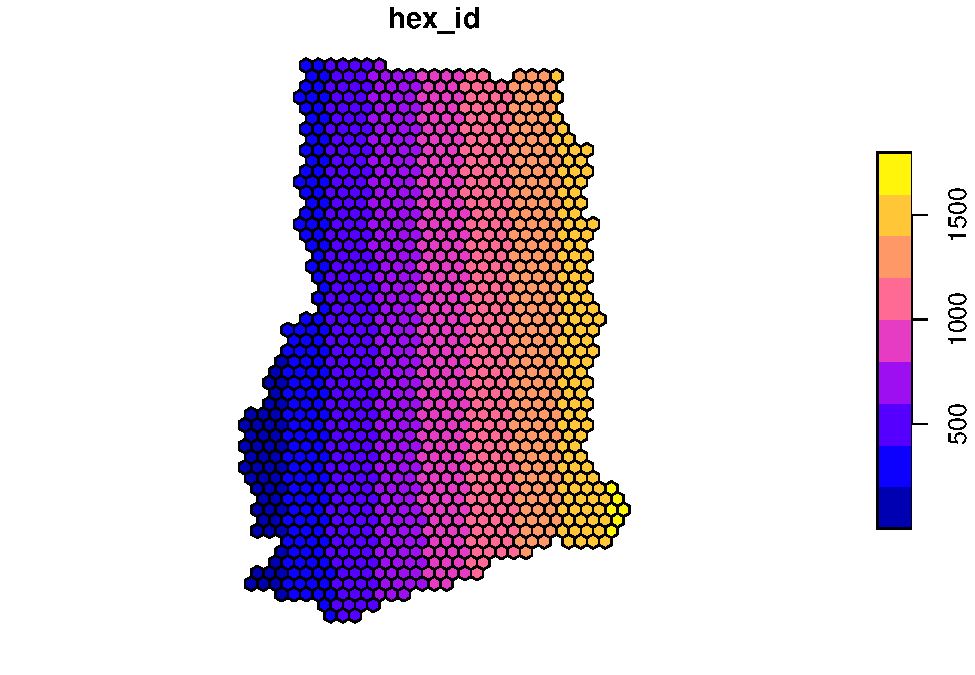
\includegraphics{unnamed-chunk-7-1.pdf}
 Now we will use the grid created above to extract the mean EVI values within
each cell for the years 2000-2020. The finer the spatial resolution, the
longer it will take, this next chunk should take 30 minutes.

\begin{Shaded}
\begin{Highlighting}[]
\CommentTok{\#This will take about 30 minutes}
\ControlFlowTok{if}\NormalTok{(}\FunctionTok{readline}\NormalTok{(}\AttributeTok{prompt =} \StringTok{"Hit enter to proceed or type \textquotesingle{}no\textquotesingle{} to download the data from G{-}Drive. "}\NormalTok{) }\SpecialCharTok{==} \StringTok{"no"}\NormalTok{)\{}
\NormalTok{googledrive}\SpecialCharTok{::}\FunctionTok{drive\_download}\NormalTok{(}\AttributeTok{file =} 
\NormalTok{                              googledrive}\SpecialCharTok{::}\FunctionTok{as\_id}\NormalTok{(}\StringTok{"https://drive.google.com/drive/folders/1ZnCpYz38ezSU1XG7ixJ2sPg\_DX7bO07J?usp=sharing"}\NormalTok{),}\AttributeTok{overwrite =}\NormalTok{ T)}
  \CommentTok{\#https://drive.google.com/drive/folders/1ZnCpYz38ezSU1XG7ixJ2sPg\_DX7bO07J?usp=sharing}
\NormalTok{evi.df }\OtherTok{\textless{}{-}} \FunctionTok{read.csv}\NormalTok{(}\StringTok{"rgee\_file\_2d44527a3b0e\_2022\_07\_28\_15\_40\_52.csv"}\NormalTok{)}
\NormalTok{evi.df }\OtherTok{\textless{}{-}}\NormalTok{ evi.df[,}\DecValTok{3}\SpecialCharTok{:}\FunctionTok{ncol}\NormalTok{(evi.df)]}
\FunctionTok{colnames}\NormalTok{(evi.df) }\OtherTok{\textless{}{-}} \FunctionTok{c}\NormalTok{(}\StringTok{\textquotesingle{}hex\_id\textquotesingle{}}\NormalTok{, stringr}\SpecialCharTok{::}\FunctionTok{str\_replace\_all}\NormalTok{(}\FunctionTok{substr}\NormalTok{(}\FunctionTok{colnames}\NormalTok{(evi.df[, }\DecValTok{2}\SpecialCharTok{:}\FunctionTok{ncol}\NormalTok{(evi.df)]), }\DecValTok{2}\NormalTok{, }\DecValTok{11}\NormalTok{), }\StringTok{"\_"}\NormalTok{, }\StringTok{"{-}"}\NormalTok{)) }\CommentTok{\#Convert dates to unambiguous format}
\NormalTok{\} }\ControlFlowTok{else}\NormalTok{ \{}
\CommentTok{\#This will take about 30 minutes}
\FunctionTok{paste0}\NormalTok{(}\FunctionTok{system.time}\NormalTok{(}\AttributeTok{expr =}\NormalTok{ aoi.evi }\OtherTok{\textless{}{-}} \FunctionTok{ee\_extract}\NormalTok{(}\AttributeTok{x =}\NormalTok{ modis.evi, }\AttributeTok{y =}\NormalTok{ hex[}\StringTok{"hex\_id"}\NormalTok{], }\AttributeTok{sf =} \ConstantTok{FALSE}\NormalTok{, }\AttributeTok{scale =} \DecValTok{250}\NormalTok{, }\AttributeTok{fun =}\NormalTok{ ee}\SpecialCharTok{$}\NormalTok{Reducer}\SpecialCharTok{$}\FunctionTok{mean}\NormalTok{(), }\AttributeTok{via =} \StringTok{"drive"}\NormalTok{, }\AttributeTok{quiet =}\NormalTok{ T))}\SpecialCharTok{/}\DecValTok{60}\NormalTok{, }\StringTok{" Minutes Elapsed. "}\NormalTok{)}
\NormalTok{evi.df }\OtherTok{\textless{}{-}} \FunctionTok{as.data.frame}\NormalTok{(aoi.evi)}
\FunctionTok{colnames}\NormalTok{(evi.df) }\OtherTok{\textless{}{-}} \FunctionTok{c}\NormalTok{(}\StringTok{\textquotesingle{}hex\_id\textquotesingle{}}\NormalTok{, stringr}\SpecialCharTok{::}\FunctionTok{str\_replace\_all}\NormalTok{(}\FunctionTok{substr}\NormalTok{(}\FunctionTok{colnames}\NormalTok{(evi.df[, }\DecValTok{2}\SpecialCharTok{:}\FunctionTok{ncol}\NormalTok{(evi.df)]), }\DecValTok{2}\NormalTok{, }\DecValTok{11}\NormalTok{), }\StringTok{"\_"}\NormalTok{, }\StringTok{"{-}"}\NormalTok{))}
\FunctionTok{write.csv}\NormalTok{(}\AttributeTok{x =}\NormalTok{ evi.df, }\AttributeTok{file =} \StringTok{"\textasciitilde{}/rgee\_file\_2d44527a3b0e\_2022\_07\_28\_15\_40\_52.csv"}\NormalTok{)\}}
\end{Highlighting}
\end{Shaded}

\begin{verbatim}
## Hit enter to proceed or type 'no' to download the data from G-Drive.
\end{verbatim}

\begin{verbatim}
## File downloaded:
\end{verbatim}

\begin{verbatim}
## * 'rgee_file_6ec1c5a3a4a_2022_08_09_20_24_48.csv'
##   <id: 1TixxHPoTd5yMAGcket3a7-IpVXhV4Uid>
\end{verbatim}

\begin{verbatim}
## Saved locally as:
\end{verbatim}

\begin{verbatim}
## * 'C:/Users/Guy/AppData/Local/Temp/Rtmp00C6CS/rgee_file_6ec1c5a3a4a.csv'
\end{verbatim}

Now we are going to perform a time series analysis on the data within
each grid cell. But first, we will work through the procedure one step
at a time.

\begin{Shaded}
\begin{Highlighting}[]
\NormalTok{evi.hw.lst }\OtherTok{\textless{}{-}} \FunctionTok{list}\NormalTok{() }\CommentTok{\#Create an empty list, this will be used to house the time series projections for each cell. }
\NormalTok{evi.dcmp.lst }\OtherTok{\textless{}{-}} \FunctionTok{list}\NormalTok{() }\CommentTok{\#Create an empty list, this will be used to house the time series decomposition for each cell.}
\NormalTok{evi.trend }\OtherTok{\textless{}{-}} \FunctionTok{data.frame}\NormalTok{(}\AttributeTok{hex\_id =}\NormalTok{ evi.df}\SpecialCharTok{$}\NormalTok{hex\_id, }\AttributeTok{na.cnt =} \ConstantTok{NA}\NormalTok{, }\AttributeTok{na.cnt.2 =} \ConstantTok{NA}\NormalTok{, }\AttributeTok{trend =} \ConstantTok{NA}\NormalTok{, }\AttributeTok{p.val =} \ConstantTok{NA}\NormalTok{, }\AttributeTok{r2 =} \ConstantTok{NA}\NormalTok{, }\AttributeTok{std.er =} \ConstantTok{NA}\NormalTok{, }\AttributeTok{trnd.strngth =} \ConstantTok{NA}\NormalTok{, }\AttributeTok{seas.strngth =} \ConstantTok{NA}\NormalTok{) }\CommentTok{\#This data frame will hold the trend data}
\NormalTok{Dates }\OtherTok{\textless{}{-}} \FunctionTok{data.frame}\NormalTok{(}\AttributeTok{date =} \FunctionTok{seq}\NormalTok{(}\FunctionTok{as.Date}\NormalTok{(}\StringTok{\textquotesingle{}2001{-}01{-}01\textquotesingle{}}\NormalTok{), }\FunctionTok{as.Date}\NormalTok{(}\StringTok{\textquotesingle{}2019{-}11{-}01\textquotesingle{}}\NormalTok{), }\StringTok{"month"}\NormalTok{))}
\NormalTok{Dates}\SpecialCharTok{$}\NormalTok{month }\OtherTok{\textless{}{-}} \FunctionTok{month}\NormalTok{(Dates}\SpecialCharTok{$}\NormalTok{date)}
\NormalTok{Dates}\SpecialCharTok{$}\NormalTok{year }\OtherTok{\textless{}{-}} \FunctionTok{year}\NormalTok{(Dates}\SpecialCharTok{$}\NormalTok{date)}
\NormalTok{i }\OtherTok{\textless{}{-}} \DecValTok{1}
\NormalTok{tsv }\OtherTok{\textless{}{-}} \FunctionTok{data.frame}\NormalTok{(}\AttributeTok{evi =} \FunctionTok{t}\NormalTok{(evi.df[i, }\DecValTok{2}\SpecialCharTok{:}\FunctionTok{ncol}\NormalTok{(evi.df)])) }\CommentTok{\#converting the data to a transposed data frame}
\FunctionTok{colnames}\NormalTok{(tsv) }\OtherTok{\textless{}{-}} \FunctionTok{c}\NormalTok{(}\StringTok{"evi"}\NormalTok{)}
\CommentTok{\#write.csv(tsv,"Data/tsv.csv")}
\FunctionTok{head}\NormalTok{(tsv) }\CommentTok{\#let\textquotesingle{}s take a look}
\end{Highlighting}
\end{Shaded}

\begin{verbatim}
##                  evi
## 2001-01-17 0.3103816
## 2001-03-22 0.6017811
## 2001-04-23 0.5585050
## 2002-01-17 0.3728227
## 2002-02-02 0.4369971
## 2002-04-07 0.5701539
\end{verbatim}

\hypertarget{method}{%
\section{Method}\label{method}}

Time series data is the collection of observations made sequentially at
different points in time.Because data points in time series are
collected at adjacent time periods there is potential for correlation
between observations. we propose some new tools to allow machine
learning classifiers to cope with time series data. We first argue that,
time-series classification problems can be solved by detecting and
combining local properties or patterns in time series. Then, a technique
is proposed to find patterns which are useful for classification. These
patterns are combined to build interpretable classification rules.
First, we will pull Sentinel 2 to select NDVI and EVI data from Google
Earth Engine,applying a quality filter to mask poor quality
pixels.Instead of performing our analysis on the imagery itself, we will
be summarizing the mean NDVI and EVI value , this will allow the
analysis to take less time while producing a visually appealing and
informative map.Some cells may not contain NDVI and EVI for a given
month, to correct this, we will apply smoothing method using an ARIMA
function. Once NA values are remove, we will decompose the time series
to remove seasonality and fit a linear model to the normalized data.
Once we have extracted the linear trend, we will then make a move to
classifier our dataon the map and map it.

\begin{Shaded}
\begin{Highlighting}[]
\NormalTok{na.cnt }\OtherTok{\textless{}{-}} \FunctionTok{length}\NormalTok{(tsv[}\FunctionTok{is.na}\NormalTok{(tsv)]) }\CommentTok{\#We want to get an idea of the number of entries with no EVI value}
\NormalTok{evi.trend}\SpecialCharTok{$}\NormalTok{na.cnt[i] }\OtherTok{\textless{}{-}}\NormalTok{ na.cnt}
\NormalTok{td }\OtherTok{\textless{}{-}}\NormalTok{ tsv }\SpecialCharTok{\%\textgreater{}\%} 
  \FunctionTok{mutate}\NormalTok{(}\AttributeTok{month =} \FunctionTok{month}\NormalTok{(}\FunctionTok{as.Date}\NormalTok{(}\FunctionTok{rownames}\NormalTok{(tsv))), }\AttributeTok{year =} \FunctionTok{year}\NormalTok{(}\FunctionTok{as.Date}\NormalTok{(}\FunctionTok{rownames}\NormalTok{(tsv)))) }\SpecialCharTok{\%\textgreater{}\%} 
  \FunctionTok{group\_by}\NormalTok{(year, month) }\SpecialCharTok{\%\textgreater{}\%}
  \FunctionTok{summarise}\NormalTok{(}\AttributeTok{mean\_evi =} \FunctionTok{mean}\NormalTok{(evi, }\AttributeTok{na.rm =}\NormalTok{ T), }\AttributeTok{.groups =} \StringTok{"keep"}\NormalTok{) }\SpecialCharTok{\%\textgreater{}\%}
  \FunctionTok{as.data.frame}\NormalTok{()}
\FunctionTok{head}\NormalTok{(td)}
\end{Highlighting}
\end{Shaded}

\begin{verbatim}
##   year month  mean_evi
## 1 2001     1 0.3103816
## 2 2001     3 0.6017811
## 3 2001     4 0.5585050
## 4 2002     1 0.3728227
## 5 2002     2 0.4369971
## 6 2002     4 0.6160278
\end{verbatim}

That looks better! Unfortunately though, there are a number of dates
which don't have any evi value at all, let's figure out which ones these
are.

\begin{Shaded}
\begin{Highlighting}[]
\NormalTok{dx}\SpecialCharTok{$}\NormalTok{mean\_evi }\OtherTok{\textless{}{-}} \ConstantTok{NA}
\NormalTok{tdx }\OtherTok{\textless{}{-}} \FunctionTok{rbind}\NormalTok{(td, dx) }\SpecialCharTok{\%\textgreater{}\%} 
  \FunctionTok{arrange}\NormalTok{(date)}
\FunctionTok{write.csv}\NormalTok{(tdx,}\StringTok{"Data/tdx.csv"}\NormalTok{)}
\NormalTok{tdx }\OtherTok{\textless{}{-}} \FunctionTok{read.csv}\NormalTok{(}\StringTok{"Data/tdx.csv"}\NormalTok{)}
\FunctionTok{head}\NormalTok{(tdx)}
\end{Highlighting}
\end{Shaded}

\begin{verbatim}
##     X year month  mean_evi       date
## 1   1 2001     1 0.3103816 2001-01-01
## 2 216 2001     2        NA 2001-02-01
## 3   2 2001     3 0.6017811 2001-03-01
## 4   3 2001     4 0.5585050 2001-04-01
## 5 510 2001     5        NA 2001-05-01
## 6 610 2001     6        NA 2001-06-01
\end{verbatim}

\begin{Shaded}
\begin{Highlighting}[]
\NormalTok{na.cnt }\OtherTok{\textless{}{-}} \FunctionTok{length}\NormalTok{(tdx[}\FunctionTok{is.na}\NormalTok{(tdx)])}
\NormalTok{evi.trend}\SpecialCharTok{$}\NormalTok{na.cnt}\FloatTok{.2}\NormalTok{[i] }\OtherTok{\textless{}{-}}\NormalTok{ na.cnt }\CommentTok{\#add count of na values to dataframe}
\FunctionTok{rm}\NormalTok{(td, dx) }\CommentTok{\#remove data we\textquotesingle{}re no longer using, this is a good rule of thumb, especially when working with larger datasets.}
\NormalTok{tdx }\OtherTok{\textless{}{-}} \FunctionTok{ts}\NormalTok{(}\AttributeTok{data =}\NormalTok{ tdx}\SpecialCharTok{$}\NormalTok{mean\_evi, }\AttributeTok{start =} \FunctionTok{c}\NormalTok{(}\DecValTok{2001}\NormalTok{, }\DecValTok{1}\NormalTok{), }\AttributeTok{end =} \FunctionTok{c}\NormalTok{(}\DecValTok{2019}\NormalTok{, }\DecValTok{11}\NormalTok{), }\AttributeTok{frequency =} \DecValTok{12}\NormalTok{) }\CommentTok{\#convert data to time series.}
\FunctionTok{plot}\NormalTok{(tdx)}
\end{Highlighting}
\end{Shaded}

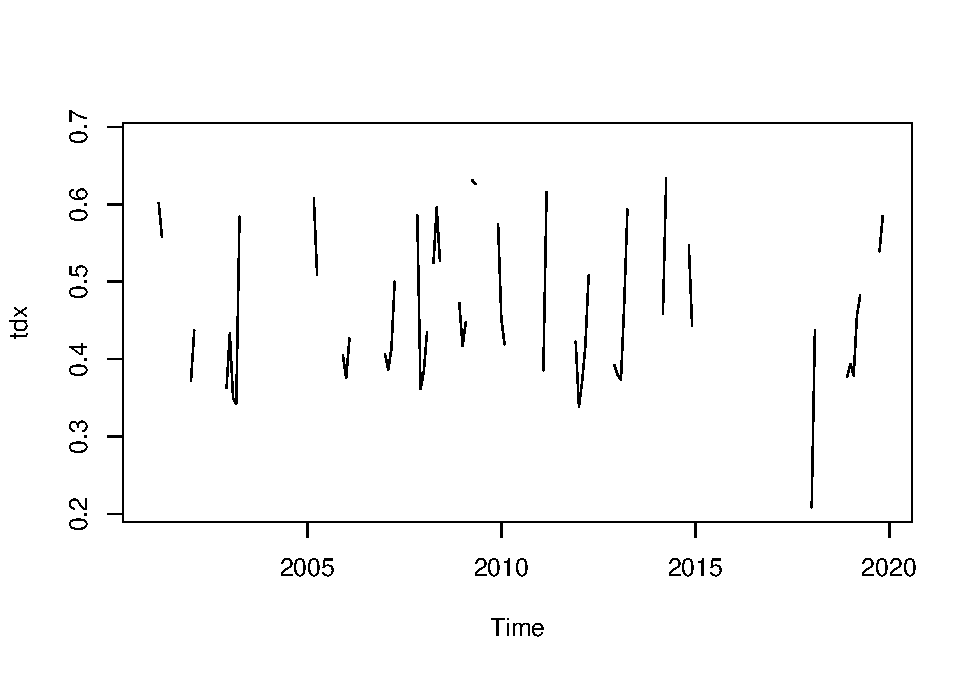
\includegraphics{unnamed-chunk-13-1.pdf}

\begin{Shaded}
\begin{Highlighting}[]
\FunctionTok{library}\NormalTok{(imputeTS)}
\NormalTok{tdx }\OtherTok{\textless{}{-}} \ControlFlowTok{if}\NormalTok{(na.cnt }\SpecialCharTok{\textgreater{}} \DecValTok{0}\NormalTok{)\{imputeTS}\SpecialCharTok{::}\FunctionTok{na\_kalman}\NormalTok{(tdx, }\AttributeTok{model =} \StringTok{"auto.arima"}\NormalTok{, }\AttributeTok{smooth =}\NormalTok{ T)\} }\ControlFlowTok{else}\NormalTok{ \{}
\NormalTok{    tdx}
\NormalTok{\}}
\FunctionTok{plot}\NormalTok{(tdx)}
\end{Highlighting}
\end{Shaded}

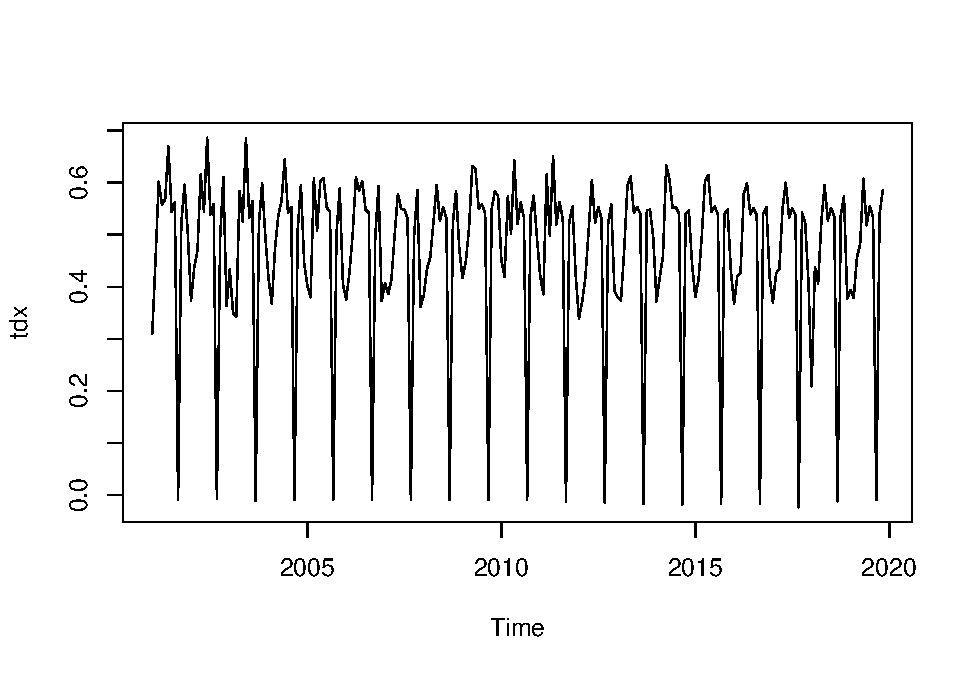
\includegraphics{unnamed-chunk-14-1.pdf}

\begin{Shaded}
\begin{Highlighting}[]
\NormalTok{tdx.dcp }\OtherTok{\textless{}{-}} \FunctionTok{stl}\NormalTok{(tdx, }\AttributeTok{s.window =} \StringTok{\textquotesingle{}periodic\textquotesingle{}}\NormalTok{)}
\FunctionTok{plot}\NormalTok{(tdx.dcp)}
\end{Highlighting}
\end{Shaded}

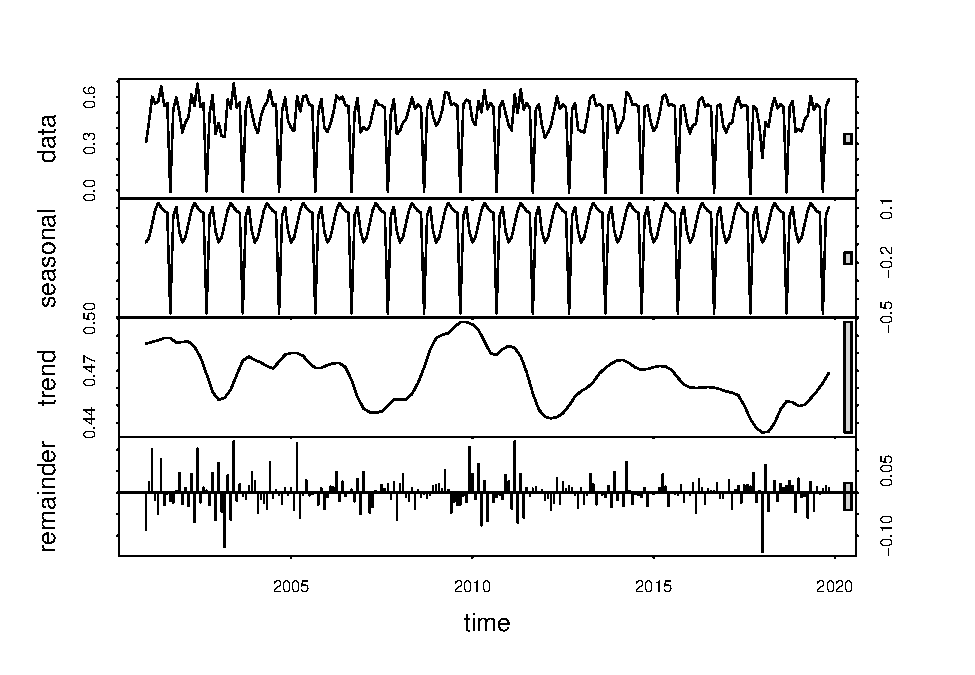
\includegraphics{unnamed-chunk-15-1.pdf}

\begin{Shaded}
\begin{Highlighting}[]
\FunctionTok{library}\NormalTok{(forecast)}
\end{Highlighting}
\end{Shaded}

\begin{verbatim}
## Warning: package 'forecast' was built under R version 4.1.3
\end{verbatim}

\begin{Shaded}
\begin{Highlighting}[]
\NormalTok{Tt }\OtherTok{\textless{}{-}} \FunctionTok{trendcycle}\NormalTok{(tdx.dcp)}
\NormalTok{St }\OtherTok{\textless{}{-}} \FunctionTok{seasonal}\NormalTok{(tdx.dcp)}
\NormalTok{Rt }\OtherTok{\textless{}{-}} \FunctionTok{remainder}\NormalTok{(tdx.dcp)}
\FunctionTok{plot}\NormalTok{(Tt)}
\end{Highlighting}
\end{Shaded}

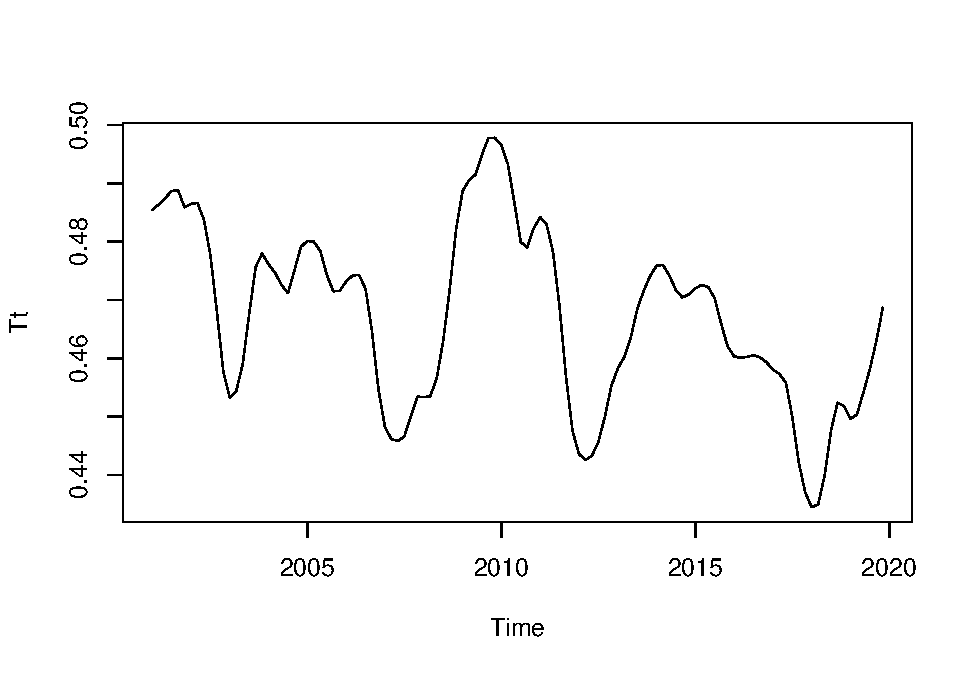
\includegraphics{unnamed-chunk-16-1.pdf}

\begin{Shaded}
\begin{Highlighting}[]
\FunctionTok{plot}\NormalTok{(St)}
\end{Highlighting}
\end{Shaded}

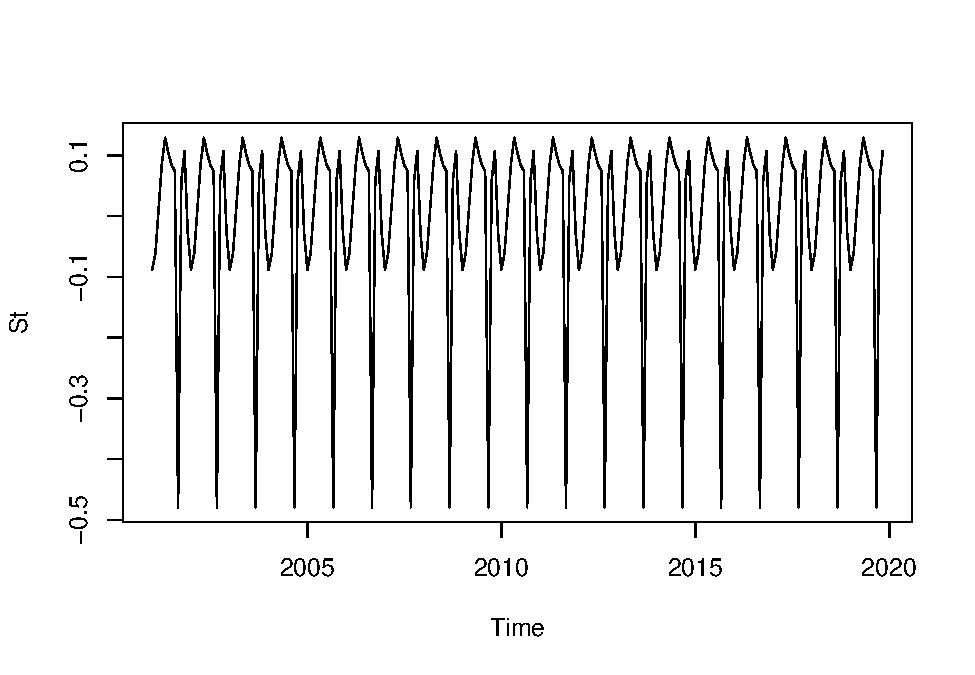
\includegraphics{unnamed-chunk-16-2.pdf}

\begin{Shaded}
\begin{Highlighting}[]
\FunctionTok{plot}\NormalTok{(Rt)}
\end{Highlighting}
\end{Shaded}

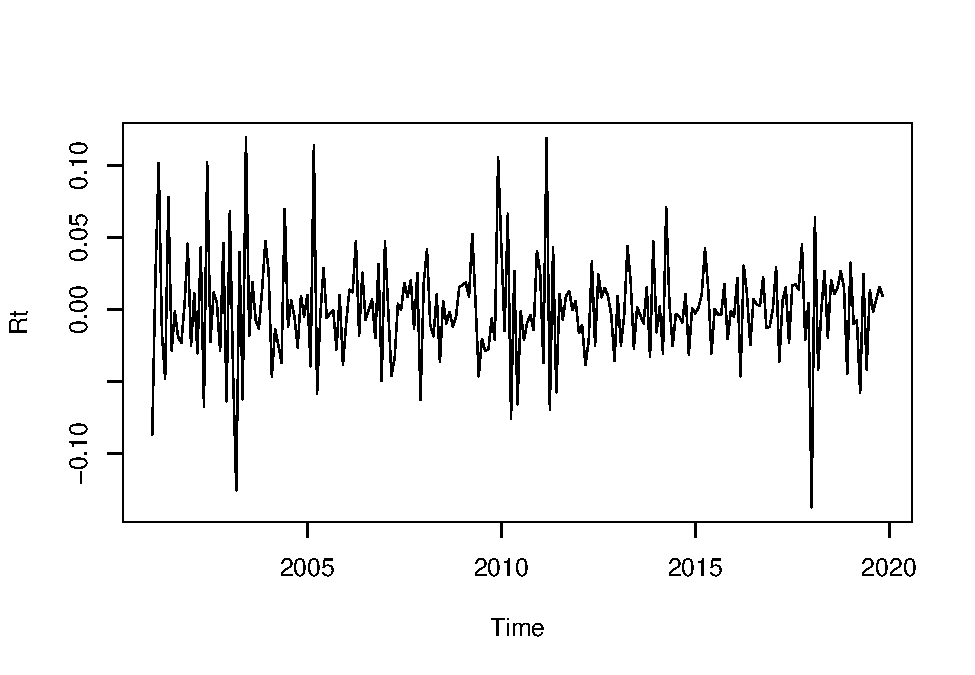
\includegraphics{unnamed-chunk-16-3.pdf}

\begin{Shaded}
\begin{Highlighting}[]
\FunctionTok{library}\NormalTok{(tseries)}
\end{Highlighting}
\end{Shaded}

\begin{verbatim}
## 
## Attaching package: 'tseries'
\end{verbatim}

\begin{verbatim}
## The following object is masked from 'package:imputeTS':
## 
##     na.remove
\end{verbatim}

\begin{Shaded}
\begin{Highlighting}[]
\FunctionTok{adf.test}\NormalTok{(Rt)}
\end{Highlighting}
\end{Shaded}

\begin{verbatim}
## 
##  Augmented Dickey-Fuller Test
## 
## data:  Rt
## Dickey-Fuller = -8.639, Lag order = 6, p-value = 0.01
## alternative hypothesis: stationary
\end{verbatim}

\begin{Shaded}
\begin{Highlighting}[]
\FunctionTok{adf.test}\NormalTok{(Tt)}
\end{Highlighting}
\end{Shaded}

\begin{verbatim}
## 
##  Augmented Dickey-Fuller Test
## 
## data:  Tt
## Dickey-Fuller = -3.4545, Lag order = 6, p-value = 0.04798
## alternative hypothesis: stationary
\end{verbatim}

\begin{Shaded}
\begin{Highlighting}[]
\NormalTok{tdx }\OtherTok{\textless{}{-}} \FunctionTok{data.frame}\NormalTok{(}\AttributeTok{time =} \FunctionTok{c}\NormalTok{(}\DecValTok{1}\SpecialCharTok{:}\FunctionTok{length}\NormalTok{(tdx)), }\AttributeTok{trend =}\NormalTok{ tdx }\SpecialCharTok{{-}}\NormalTok{ tdx.dcp}\SpecialCharTok{$}\NormalTok{time.series[,}\DecValTok{1}\NormalTok{])}
\NormalTok{trend.summ }\OtherTok{\textless{}{-}} \FunctionTok{summary}\NormalTok{(}\FunctionTok{lm}\NormalTok{(}\AttributeTok{formula =}\NormalTok{ trend }\SpecialCharTok{\textasciitilde{}}\NormalTok{ time, }\AttributeTok{data =}\NormalTok{ tdx))}
\NormalTok{trend.summ}
\end{Highlighting}
\end{Shaded}

\begin{verbatim}
## 
## Call:
## lm(formula = trend ~ time, data = tdx)
## 
## Residuals:
##       Min        1Q    Median        3Q       Max 
## -0.159773 -0.020549  0.000499  0.016519  0.135949 
## 
## Coefficients:
##               Estimate Std. Error t value Pr(>|t|)    
## (Intercept)  4.798e-01  5.293e-03  90.635  < 2e-16 ***
## time        -1.118e-04  4.026e-05  -2.778  0.00593 ** 
## ---
## Signif. codes:  0 '***' 0.001 '**' 0.01 '*' 0.05 '.' 0.1 ' ' 1
## 
## Residual standard error: 0.03974 on 225 degrees of freedom
## Multiple R-squared:  0.03317,    Adjusted R-squared:  0.02887 
## F-statistic: 7.718 on 1 and 225 DF,  p-value: 0.005928
\end{verbatim}

\begin{Shaded}
\begin{Highlighting}[]
\FunctionTok{plot}\NormalTok{(tdx)}
\FunctionTok{abline}\NormalTok{(}\AttributeTok{a =}\NormalTok{ trend.summ}\SpecialCharTok{$}\NormalTok{coefficients[}\DecValTok{1}\NormalTok{,}\DecValTok{1}\NormalTok{], }\AttributeTok{b =}\NormalTok{ trend.summ}\SpecialCharTok{$}\NormalTok{coefficients[}\DecValTok{2}\NormalTok{,}\DecValTok{1}\NormalTok{], }\AttributeTok{col =} \StringTok{\textquotesingle{}blue\textquotesingle{}}\NormalTok{)}
\end{Highlighting}
\end{Shaded}

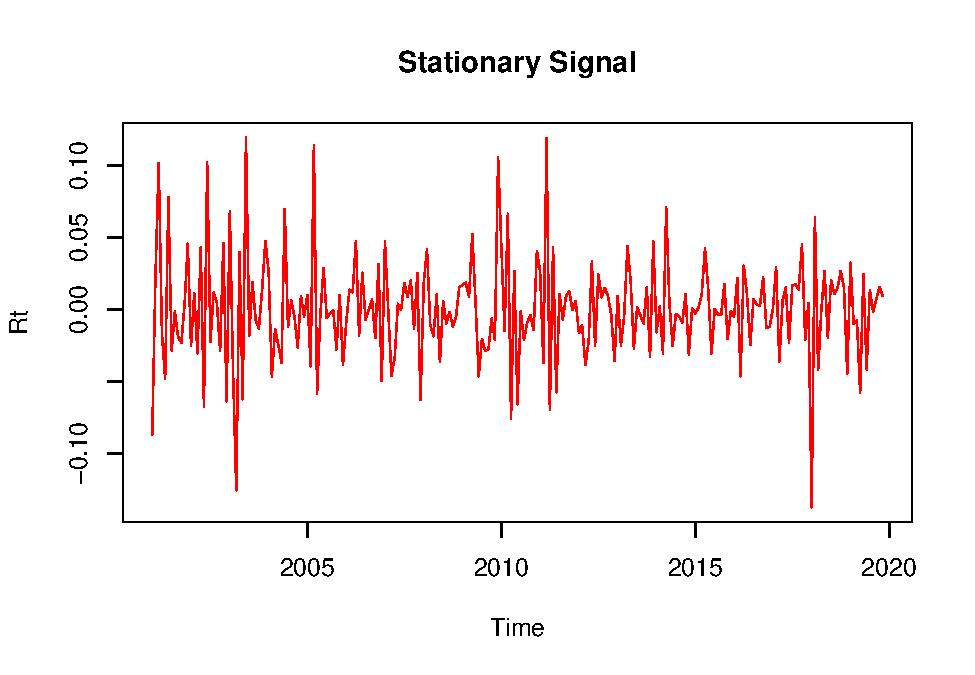
\includegraphics{unnamed-chunk-18-1.pdf}

\hypertarget{finding}{%
\subsection{Finding}\label{finding}}

\end{document}
